МРНТИ 20.15.05;81.93.29

\textbf{A COMPREHENSIVE APPROACH TO ENHANCING THE RESILIENCE OF}

\textbf{INFORMATION SYSTEMS: FROM MATHEMATICAL MODELING TO RISK
MANAGEMENT STRATEGIES}

\textbf{\textsuperscript{1, 2}Ye. Kaiupov,
\textsuperscript{2}A.Mukanova, \textsuperscript{2}A.Nazyrova,
\textsuperscript{1}B.Tashtai, \textsuperscript{1}T.Toleubekov}

\textsuperscript{1}L.N. Gumilyov Eurasian National University, Astana,
Kazakhstan,

\textsuperscript{2}Аstana International University, Astana, Kazakhstan,

e-mail: yerik.kai@gmail.com

This article discusses the issue of improving the reliability of
information systems. The main focus is on mathematical analysis methods
used to assess fault tolerance in data exchange systems. In the modern
world, when data is becoming an increasingly valuable asset, the
importance of reliability of information systems cannot be
overestimated. The research focuses on the development of a mathematical
model, which is presented in the form of a graph of states and failure
probabilities, and also includes a set of differential equations to
describe the dynamics of the system. This model is designed to operate
at three levels, which allows you to analyze in detail various aspects
of the functioning of the system and identify potential threats at each
stage.

The solution of the proposed equations allows not only to determine the
probability of failures at different points in time, but also provides
tools for effective troubleshooting. Thus, the implementation of the
proposed approach contributes to improving the overall reliability of
systems, reduces the risks of critical failures, and improves
infrastructure management. The article also discusses the possibilities
of practical application of the developed model in various types of
information systems, including critical infrastructures, where a high
level of reliability is absolutely necessary.

\textbf{Keywords:} information system, diagnostics of network
parameters, network resources reliability, failure, network operation
level.

\textbf{АҚПАРАТТЫҚ ЖҮЙЕЛЕРДІҢ ТҰРАҚТЫЛЫҒЫН АРТТЫРУДЫҢ КЕШЕНДІ ТӘСІЛІ:
МАТЕМАТИКАЛЫҚ МОДЕЛЬДЕУДЕН ТӘУЕКЕЛДЕРДІ БАСҚАРУ}

\textbf{СТРАТЕГИЯСЫНА ДЕЙІН}

\textbf{\textsuperscript{1, 2}Е.Қайупов, \textsuperscript{2}Ә.Мұқанова,
\textsuperscript{2}А.Назырова,\textsuperscript{1}Б.Таштай,
\textsuperscript{1}Т.Төлеубеков}

\textsuperscript{1}Л.Н. Гумилев атындағы Еуразия ұлттық университеті,
Астана, Қазақстан,

\textsuperscript{2}Астана халықаралық университеті, Астана, Қазақстан,

e-mail: yerik.kai@gmail.com

Бұл мақалада ақпараттық жүйелердің сенімділігін арттыру мәселесі
қарастырылады. Деректер алмасу жүйелеріндегі ақауларға төзімділікті
бағалау үшін қолданылатын математикалық талдау әдістеріне назар
аударылады. Қазіргі әлем жағдайында, деректер барған сайын құнды активке
айналған кезде, ақпараттық жүйелердің сенімділігінің маңыздылығын асыра
бағалау мүмкін емес. Зерттеу сәтсіздіктердің күйлері мен
ықтималдықтарының графигі ретінде ұсынылған математикалық модельді
әзірлеуге бағытталған, сонымен қатар, жүйенің динамикасын сипаттайтын
дифференциалдық теңдеулер кешенін қамтиды. Бұл модель жүйенің жұмыс
істеуінің әртүрлі аспектілерін егжей-тегжейлі талдауға және әр кезеңдегі
ықтимал қауіптерді анықтауға мүмкіндік беретін үш деңгейде жұмыс істеуге
арналған.

Ұсынылған теңдеулерді шешу уақыттың әртүрлі нүктелерінде ақаулардың
пайда болу ықтималдығын анықтауға ғана емес, сонымен қатар, ақаулықтарды
тиімді анықтауға және жоюға арналған құралдарды ұсынады. Осылайша,
ұсынылған тәсілді енгізу жүйелердің жалпы сенімділігін арттыруға ықпал
етеді, маңызды істен шығу қаупін азайтады және инфрақұрылымды басқаруды
жақсартады. Мақалада сонымен қатар, сенімділіктің жоғары деңгейі өте
қажет болатын маңызды инфрақұрылымдарды қоса алғанда, ақпараттық
жүйелердің әртүрлі түрлерінде әзірленген модельді практикалық қолдану
мүмкіндіктері талқыланады.

\textbf{Түйін сөздер:} ақпараттық жүйе, желі параметрлерінің
диагностикасы, желілік ресурстардың сенімділігі, істен шығуы, желінің
жұмыс деңгейі.

\textbf{КОМПЛЕКСНЫЙ ПОДХОД К ПОВЫШЕНИЮ УСТОЙЧИВОСТИ ИНФОРМАЦИОННЫХ
СИСТЕМ: ОТ МАТЕМАТИЧЕСКОГО МОДЕЛИРОВАНИЯ ДО СТРАТЕГИЙ УПРАВЛЕНИЯ
РИСКАМИ}

\textbf{\textsuperscript{1,2}Е.Кайупов, \textsuperscript{2}А.Муканова,
\textsuperscript{2}А.Назырова, \textsuperscript{2}Б.Таштай,
\textsuperscript{2}Т.Толеубеков}

\textsuperscript{1}Евразийский национальный университет имени Л.Н.
Гумилева, Астана, Казахстан,

\textsuperscript{2} Международный университет Астана, астана, Казахстан,

e-mail: yerik.kai@gmail.com

В данной статье рассматривается вопрос повышения надежности
информационных систем. Основное внимание уделяется методам
математического анализа, применяемым для оценки устойчивости к сбоям в
системах обмена данными. В условиях современного мира, когда данные
становятся все более ценным активом, важность надежности информационных
систем не может быть переоценена. Исследование фокусируется на
разработке математической модели, которая представлена в виде графика
состояний и вероятностей отказов, а также включает комплекс
дифференциальных уравнений для описания динамики системы. Эта модель
разработана для функционирования на трех уровнях, что позволяет детально
анализировать различные аспекты функционирования системы и
идентифицировать потенциальные угрозы на каждом из этапов.

Решение предложенных уравнений позволяет не только определить
вероятности возникновения сбоев в разные моменты времени, но и
предоставляет инструменты для эффективного выявления и устранения
неисправностей. Таким образом, внедрение предложенного подхода
способствует повышению общей надежности систем, снижает риски
возникновения критических отказов, и улучшает управление
инфраструктурой. В статье также обсуждаются возможности практического
применения разработанной модели в различных типах информационных систем,
включая критически важные инфраструктуры, где высокий уровень надежности
является абсолютно необходимым.

\textbf{Ключевые слова:} информационная система, диагностика параметров
сети, надежность сетевых ресурсов, отказы, уровень функционирования
сети.

\textbf{Introduction.} In the modern world, where information technology
plays a leading role in various spheres of human activity, the
reliability of information systems becomes a critically important
aspect. These systems form the basis for data transmission, processing,
and storage, and any malfunctions in their operation can lead to serious
consequences, including data loss, reduced productivity, and even
critical emergency situations in vital infrastructures. Therefore,
enhancing the resilience of information systems to failures and
malfunctions is a priority task for specialists in the field of
information technology.

The problem of information system reliability is multifaceted and
requires a comprehensive approach to its solution. In recent years,
methods of mathematical modeling have been actively developed, allowing
the analysis and prediction of system behavior under various external
and internal influences. The application of these methods opens new
possibilities for assessing fault tolerance and developing effective
strategies to enhance the reliability of information systems.

This article proposes an innovative method for assessing the resilience
of information systems to failures, based on mathematical modeling. The
method includes the development of a mathematical model, which is a
graph of states and failure probabilities, as well as a system of
differential equations for its description. This model allows for the
identification of potential vulnerabilities in the structure and
functioning of information systems, as well as aids in the development
of measures to eliminate them. The solution of the proposed model
provides quantitative estimates of failure probabilities at various
levels of system operation, which is a key element in ensuring its
reliability.

The article is organized as follows: after an introduction that outlines
the relevance of the problem and the goals of the research, a literature
review reflects the current state of the issue of assessing the
reliability of information systems. The methodology for developing the
mathematical model, the main stages of its creation, and the principles
of operation are then described. The results section presents the data
obtained during the modeling and their analysis. The conclusion
summarizes the findings of the research and outlines prospects for
further work in this area.

\textbf{Materials and methods.} To assess the resilience of information
systems to failures, methods of mathematical analysis and mathematical
modeling were used, including the development of a state graph and
failure probabilities, as well as a system of differential equations for
analyzing and optimizing the functioning of systems across three levels:
data transmission, processing, and storage. This allowed for the
prediction of failure probabilities and the identification of critical
points to enhance system reliability.

\textbf{Literature Review.} Extensive research has been conducted in the
field of hardware protection against malfunctions and system security,
presented in a series of key articles. One of the innovative
developments is S-DETECTOR, introduced in {[}1{]}, which is an
implementation of DETECTOR with selective protection of vulnerable
registers. This approach significantly enhances performance and also
reduces the damage that could be caused by failure coverage.

In the field of electric vehicles, a collision prevention system is
actively being developed, introduced in {[}2{]}. This method is
innovative due to the use of embedded real-time subsystems at the
hardware level, providing reliable protection against potential faults.

The fundamental methodology for designing fault-tolerant microprocessor
systems, described in {[}3{]}, is based on software-implementable
hardware fault tolerance. This methodology represents an important step
towards creating systems capable of effectively dealing with potential
malfunctions and ensuring reliable operation.

Article {[}4{]} proposes an extension of the scheduling theory for
mixed-criticality systems, taking into account temporal faults. These
extensions, which introduce the concept of discard relations
generalizing the notion of criticality, aim to improve the
schedulability analysis and the control of dependencies between tasks,
facilitating effective system resource management and enhancing
reliability in the face of temporal faults.

Experimental data presented in {[}5{]} demonstrate that the Defender
architecture for a fault-tolerant router in a network-on-chip
successfully ensures resilience to permanent faults. Other studies, such
as the use of approximate computations to reduce energy consumption in
deep neural network accelerators {[}6{]} and a design methodology for
enhancing the fault tolerance of deep learning models using neuromorphic
hardware {[}8{]}, also make significant contributions to the field of
hardware protection.

Furthermore, article {[}7{]} examines the Defender architecture for a
fault-tolerant router in a network-on-chip, marking an important step in
ensuring resilience to permanent faults in modern network systems.

In the context of secure multicast in networks with interceptors,
article {[}9{]} explores the issue and develops methods for ensuring
security in environments with multiple sources.

Detailed studies, such as proving security for the two-message signed
Diffie-Hellman key exchange protocol {[}10{]}, and the extended
mechanism for ensuring integrity and predictability in intra-chip
communication during random hardware faults (AIQ) {[}11{]}, provide a
deep analysis and development of tools for cybersecurity in modern
computing environments.

A review of contemporary trends in access control in the Internet of
Things (IoT) {[}12{]} makes an important contribution to understanding
security in the realm of device and system interactions in the IoT.

Research such as the use of CSP process algebra and the PAT tool for
analyzing the Apache Kafka messaging mechanism {[}13{]}, as well as a
review of the security of existing Digital Signature Schemes (DSS) in
the context of the strong existential unforgeability under chosen
message attack model (sEUF-CMA) {[}14{]}, provide valuable knowledge for
ensuring security in the realms of data exchange and signatures.

Considering the advancement of modern technologies, studies on the
application of a new protocol with a guaranteed error of O(1/ε) for pure
differential privacy {[}15{]} and examining the security of the Signal
messenger with a proposal for an improved protocol SAID {[}16{]} offer
new perspectives and solutions for secure data transmission and
communications.

Finally, research in the field of distributed systems, such as a
Configurable Distributed System for Verification and Launch (CDCLS) for
aerospace vehicles {[}17{]} and the proposal of the DepFast library
{[}18{]}, are significant steps in the field of ensuring fault tolerance
and efficient resource management in modern distributed systems
{[}19{]}.

This literature review also addresses issues of processing large volumes
of data in intelligent transportation using mobile edge computing
technology {[}20{]}. Challenges related to efficient data management and
processing in transportation systems are becoming increasingly relevant,
and this research suggests approaches to addressing these challenges
based on the use of mobile computing.

Additionally, considering a secure data transmission mechanism in ad hoc
mobile networks {[}21{]} is an important part of the review. Ensuring
secure data transmission in ad hoc networks, where devices interact
without a centralized infrastructure, is a complex task, and this
article suggests approaches to ensuring confidentiality and integrity of
data in such networks.

Research on Scalable Multilevel Distributed Coding (SMDC) for encoding
independent information messages with different reliability requirements
{[}22{]} also contributes to the discussion on fault tolerance and
security. This approach can be useful for transmitting information under
conditions where different messages have varying reliability
requirements.

In conclusion, introducing a new steganography model - the Cover
Processing-based Steganographic Model (CPSM) {[}23{]} - complements the
discussion on innovative approaches to ensuring confidentiality and
security of information messages. This model offers new ways of
embedding and protecting information, making it significant in the
context of developing secure messaging systems.

\textbf{Modeling Object.} The object of modeling in the scientific
article presented is information systems designed to ensure the
transmission, processing, and storage of data in various areas of human
activity. Particular attention is paid to data transmission systems
operating under increased reliability and fault tolerance requirements.
The study aims to analyze and assess the resilience of these systems to
potential failures and malfunctions that may arise due to various
external and internal impacts.

As a specific object of modeling, information systems with a three-level
operating architecture are chosen, including data transmission, data
processing, and data storage levels. This structure reflects the
complexity and hierarchy of modern information systems and allows for
considering various scenarios of system component interactions and their
impact on overall reliability.

A mathematical model based on graph theory and probability theory
principles has been developed to analyze the fault tolerance of
information systems. The model is a state graph, each state
corresponding to a certain level of system operation, and transition
probabilities between these states, reflecting the likelihood of system
component failures and their impact on overall operability. A system of
differential equations is used to describe the dynamics of system state
changes, the solution of which allows estimating the probabilities of
the system being in each of the possible states over time.

Modeling the fault tolerance of information systems using the proposed
mathematical model enables the identification of the most vulnerable
elements of the system, assess the risks of potential failures, and
develop strategies to improve reliability and resilience to
malfunctions. This approach ensures a higher level of information
systems\textquotesingle{} readiness for unforeseen situations, minimizes
potential losses from failures and malfunctions, and improves the
quality of service for end-users.

Table 1 presents the critically important components of information
systems (IS), their main functions, and the level of criticality.

\textbf{Table 1 - Important components of Information systems (IS)}

\begin{longtable}[]{@{}
  >{\raggedright\arraybackslash}p{(\columnwidth - 6\tabcolsep) * \real{0.0640}}
  >{\raggedright\arraybackslash}p{(\columnwidth - 6\tabcolsep) * \real{0.3227}}
  >{\raggedright\arraybackslash}p{(\columnwidth - 6\tabcolsep) * \real{0.4171}}
  >{\raggedright\arraybackslash}p{(\columnwidth - 6\tabcolsep) * \real{0.1962}}@{}}
\toprule\noalign{}
\begin{minipage}[b]{\linewidth}\raggedright
\textbf{№}
\end{minipage} & \begin{minipage}[b]{\linewidth}\raggedright
\textbf{Component}
\end{minipage} & \begin{minipage}[b]{\linewidth}\raggedright
\textbf{Function}
\end{minipage} & \begin{minipage}[b]{\linewidth}\raggedright
\textbf{Criticality Level}
\end{minipage} \\
\midrule\noalign{}
\endhead
\bottomrule\noalign{}
\endlastfoot
1 & Database Server & Data storage, management, and processing & High \\
2 & Communication Equipment & Ensuring data transmission between network
devices & Medium \\
3 & Application Server & Running business applications and services &
High \\
4 & Data Storage Systems & Centralized storage of large volumes of data
& High \\
5 & Backup Systems & Data recovery after failures & High \\
6 & Network Routers and Switches & Traffic routing and network flow
management & Medium \\
7 & Security Systems (Firewall, IDS/IPS) & Network protection against
unauthorized access and attacks & High \\
8 & Data Processing Centers (DPC) & Physical and software support of IT
infrastructure & High \\
9 & End-User Devices (PCs, Laptops) & User access to applications and
data & Medium \\
10 & Cloud Computing Services & Flexible scaling and resource
provisioning & Medium \\
\end{longtable}

This classification emphasizes the importance of various IS components
in ensuring their stable and reliable operation. Components with a high
level of criticality require special attention in the context of
developing measures to improve fault tolerance and ensure data security.

The functional state of an information system (IS) can be represented in
accordance with Figure 1, where the efficiency of the IS is determined
by its ability and readiness to perform basic functions, such as sending
data packets and processing user requests. In contrast to efficient
operation, an inefficient state of the IS is characterized by problems
including delays, malfunctions, and complete failures. Additionally,
within the scope of the study, various categories of errors that can
lead to system failures can be identified, as detailed in Figure 2.

\begin{figure}[H]
	\centering
	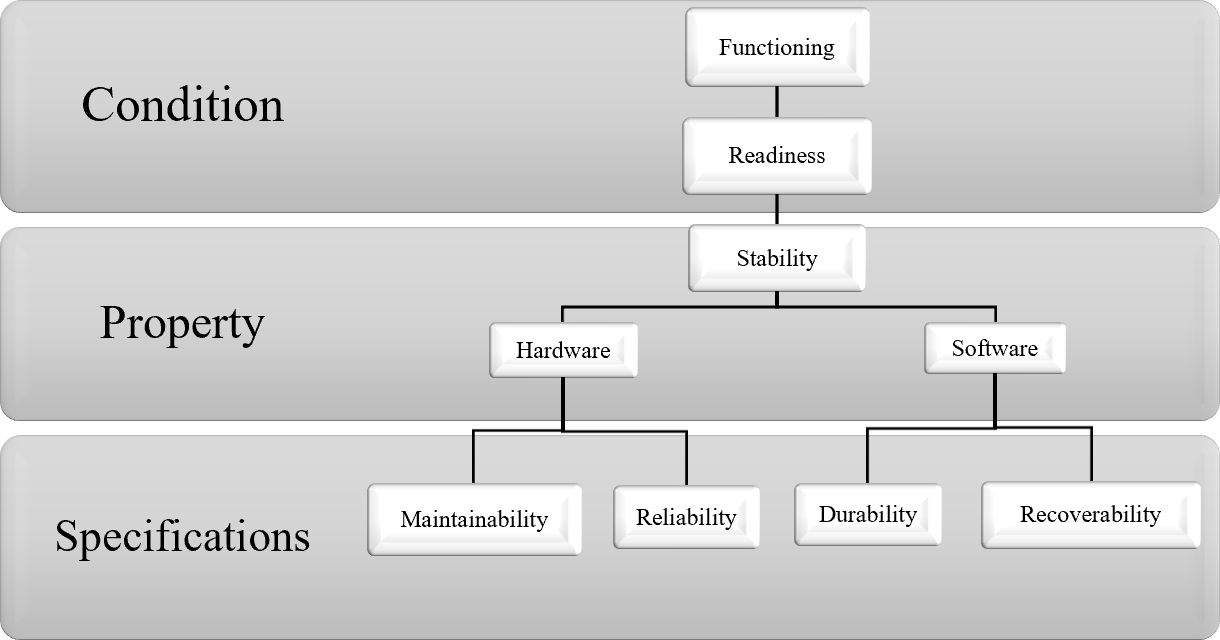
\includegraphics[width=0.8\textwidth]{assets/43}
	\caption*{}
\end{figure}

\textbf{Figure 1 - Characteristics of the functioning of the IS}

\begin{figure}[H]
	\centering
	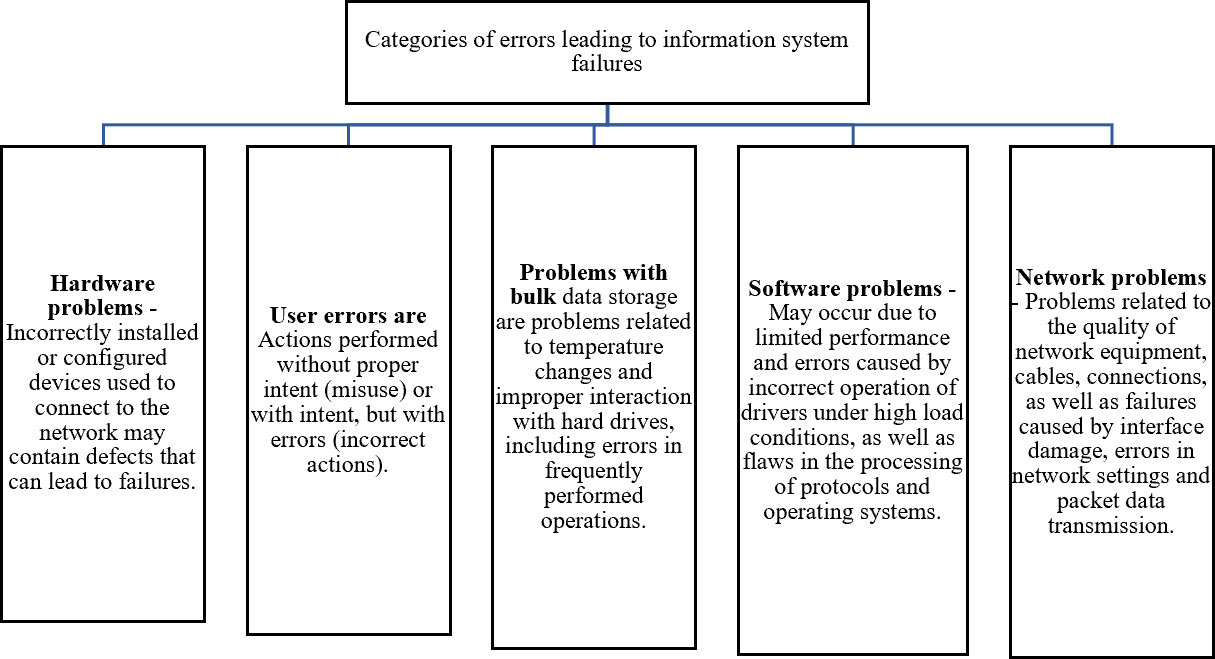
\includegraphics[width=0.8\textwidth]{assets/44}
	\caption*{}
\end{figure}

\textbf{Figure 2 - Errors that can lead to failures And}

In the framework of system-technical analysis, information systems are
considered as integrated structures consisting of interconnected and
interacting levels. The key elements of such systems are system and
application software, database management systems, as well as a set of
functions and services responsible for data transmission, storage and
processing (Figure 3).

\begin{figure}[H]
	\centering
	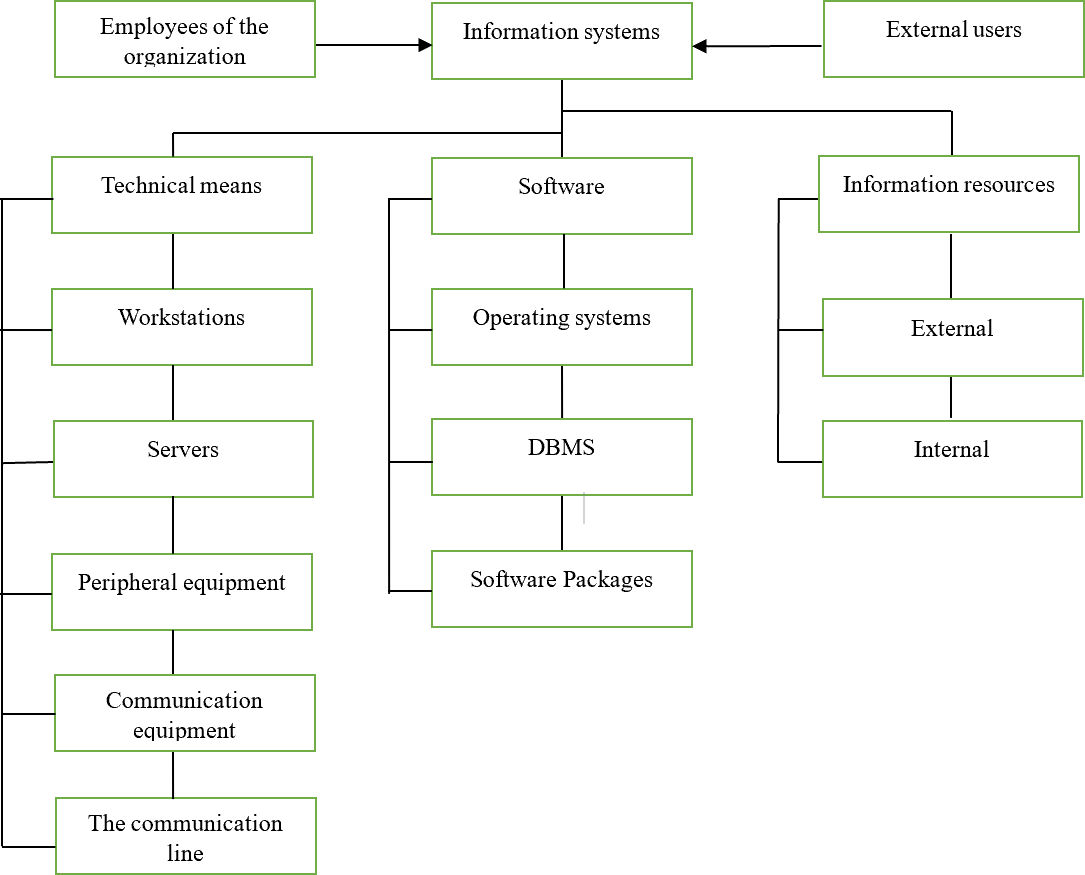
\includegraphics[width=0.8\textwidth]{assets/45}
	\caption*{}
\end{figure}

\textbf{Figure 3- Information systems}

When developing reliable and fault-tolerant information systems and
networks, significant attention is dedicated to minimizing the time and
resources required for the recovery and replacement of failed
components. In light of this, the application of various modeling
methods for selecting the optimal strategy for implementing backup
elements, considering potential failures, becomes a highly sought-after
approach.

The task of modeling and assessing the probabilities of failures in
information systems acquires particular relevance, allowing for the
identification of components that require modernization or replacement
with backups. For addressing this task, it is appropriate to use the
Markov chain methodology. This method is one of the most accessible and
effective mathematical tools for modeling various operations, including
failures in information systems, occurring as random processes.

Markov chains are an established mathematical tool for analyzing
problems with a probabilistic nature. Such a chain is represented in the
form of a graph, where vertices correspond to system states, and edges
reflect the intensity of transitions between these states. Using an
annotated graph, it is possible to determine the probabilities of the
system being in each of the states both over time and in stationary
conditions.

Before beginning modeling, initial parameters are defined, such as
possible states of failures specific to the analyzed information system,
and all potential connections between states are established in the form
of event flow intensities that effectuate the system\textquotesingle s
transitions from one state to another.

Then, based on the set parameters, one can proceed to create the model
using graph methodology, based on the principles of Markov chain theory.

In the context of the analyzed information system, a failure is
considered a stochastic process with a finite set of states, where
events occur individually rather than en masse. This indicates the
ordinariness of the studied model, which also assumes the absence of
aftereffects. This means that the number of events occurring in any
given time interval does not correlate with the number of events in any
other non-overlapping interval.

In the process of building the model to assess network fault tolerance,
it is assumed that a failure can occur at any level of its operation at
any given time, including the local level, the network environment
level, or the level of system\textquotesingle s critically significant
nodes (Figure 4).

\begin{figure}[H]
	\centering
	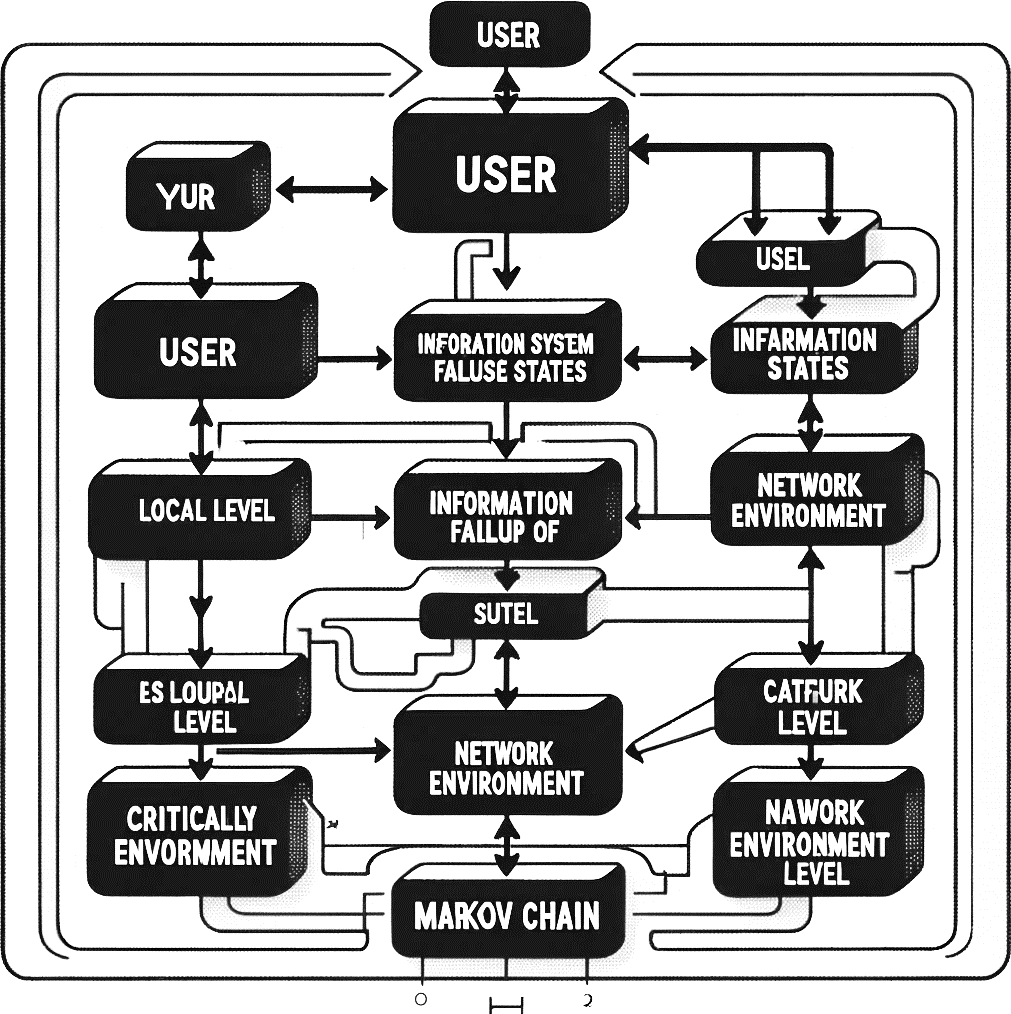
\includegraphics[width=0.8\textwidth]{assets/46}
	\caption*{}
\end{figure}

\textbf{Figure 4 - Schematic representation of the hierarchy of failure
states of an information system with}

\textbf{modeling based on Markov chains}

In the process of developing a model and evaluating the characteristics
of network fault tolerance, it is assumed that the information system at
certain points in time may experience a failure at one of the levels of
its functioning. These levels include: the local level, the network
environment level, and the critical node level. Within the framework of
modeling, it is assumed that the system can be in various failure
states, designated as Sij, where the index i indicates the level of
functioning (with three levels in this example), and the index j
classifies the type of failure (with five different types in this
example).

The initial state of the system is assumed to be trouble-free, with
fully functioning resources. All subsequent states differ from the
initial one and are characterized by non-standard operation of the
system in conditions of various failures.

Next, a graph of system states is constructed, which illustrates the
transitions from each possible failure state at the appropriate level to
a failure-free state, designated as S0. In this graph, the vertices
represent the possible states of the system, and the edges reflect the
intensity of transitions between these states, denoted as λi.

To quantify fault tolerance and failure probabilities in the network, a
mathematical model is formed based on the constructed graph of states.
This model is expressed through a system of differential or linear
algebraic equations, following the rule: on the left is the derivative
of the probability of a state in time, and on the right is the sum of
the products of the probabilities of states from which transitions to a
given state occur, based on the intensity of the corresponding streams
of events, minus the total intensity of the streams leading away from
this state, multiplied by the probability of this state.

To assess the level of fault tolerance and find the probabilities of
failures in the network according to a structured graph, we compile a
mathematical model in the form of a system of differential or linear
algebraic equations according to the following rule: on the left is the
derivative of the probability of the state, and on the right is the sum
of the products of the probabilities of those states from which the
arrows go to this state, based on the intensity of the corresponding
event flows, minus the total intensity of the flows leading from a given
state multiplied by the probability of a given state

To quantify the fault tolerance of the network and determine the
probability of failures, a mathematical model based on the constructed
graph of states is used. The model is presented in the form of a system
of differential or linear algebraic equations, which are formulated as
follows:

The left side of the equation contains the derivative of the probability
of finding the system in a given state in time, which corresponds to the
rate of change in the probability of this state.

The right side of the equation consists of two parts:

The first part includes the sum of the products of the probabilities of
previous states on the intensity of the streams of events that transfer
the system to this state. This reflects the contribution to the
probability of a state from all possible previous states.

The second part is the product of the probability of the current state
by the total intensity of the streams of events that bring the system
out of this state. This expresses the loss of probability due to
transitions to other states.

Thus, if we denote the probability of the \(S_{i}\) state as
\(P(S_{i})\) and the intensity of the transition from the \(S_{i}\)
state to the \(S_{j}\ \)state as \(\lambda_{ij}\), then for each
\(S_{i}\) state the equation will take the form:

\[\frac{dP(S_{i})}{dt} = \sum_{j \neq i}^{}{P(S_{j})}\lambda_{ji} - P(S_{i})\sum_{j \neq i}^{}\lambda_{ij}\]

where \(\frac{dP(S_{i})}{dt}\) - is the rate of change in the
probability of the \(S_{i}\) state over time, the first term sums up the
contributions from all possible transitions to the \(S_{i}\) state, and
the second term subtracts the probability of leaving the Si state to all
other states.

Solving this system of equations will allow us to find the probabilities
of all states of the system at any given time or in a stationary mode,
if we consider the long-term behavior of the system.

\textbf{Discussion.} In the framework of modern research, an analysis of
the fault tolerance of information systems (IS) using the theory of
Markov chains has been carried out. The central part of the work is the
construction of an IC failure graph, which describes the probabilistic
transitions between different states of the system, including states
characterizing various levels of functioning and types of failures.
Failure states in this context are divided into three main categories:
the local level, the network environment level and the level of critical
nodes, each of which, in turn, is associated with five types of
failures, covering hardware, system, application problems, as well as
failures of network devices and physical communication channels.

The study begins with determining the initial state of the system,
assuming its full functionality without any failures. The subsequent
analysis focuses on modeling the transitions of the system to failure
states and back, using a mathematical model based on Markov circuits.
This approach allows us to quantify the probabilities of each of the
possible states of the system over time, which is a key aspect in
studying and improving its fault tolerance.

In the course of the study, a system of differential and linear
algebraic equations was developed, which allows us to calculate the
dynamics of changes in the probabilities of system states based on the
intensities of event flows leading to failures or restoration of
functioning. The solution of this system of equations makes it possible
to predict the behavior of the system in various operating conditions
and under various failure scenarios.

One of the most important results of the work was the identification of
key factors affecting the level of fault tolerance of the information
system. In addition, the most vulnerable components and levels of
functioning of the IC were identified, for which the risk of failure is
maximum. This data can be used in the development of strategies to
improve the reliability and fault tolerance of systems, as well as in
planning measures to prevent failures or minimize their consequences.

\textbf{Results.} As part of the research, a mathematical model based on
Markov chains was developed and tested to analyze the fault tolerance of
information systems (IS). The model allowed us to estimate the
probabilities of transitions between different states of the system,
including normal operation and various failure levels associated with
the local level, the level of the network environment and the level of
critical nodes. The failure specification included hardware problems,
system failures, application problems, failures of network devices and
physical communication channels.

The main results of the study can be summarized as follows:

Quantification of the probabilities of states - the probabilities of
finding the system in each of the possible states were determined
depending on the time and operating conditions. This made it possible to
identify the most vulnerable components of the IC to failures and
evaluate the effectiveness of various strategies to increase fault
tolerance.

Identification of key fault tolerance factors - the study showed that
the intensity and probability of failures significantly depend on the
level of functioning of the system components and the type of possible
failures. Identifying these dependencies allows you to focus efforts on
eliminating the most significant vulnerabilities.

Analysis of the dynamics of changes in system states - the proposed
approach made it possible to trace how the probability of finding a
system in certain failure states changes over time, which contributes to
a better understanding of the recovery processes after failures and
planning preventive measures.

Development of recommendations to improve fault tolerance - based on the
results obtained, recommendations were formulated to improve the
architecture and configuration of information systems aimed at reducing
the likelihood of failures and minimizing their consequences.

Thus, the results of this study make a significant contribution to the
theory and practice of designing and operating fault-tolerant
information systems. The use of mathematical modeling based on Markov
chains allows for a more in-depth analysis of the processes taking place
in the IP and the development of effective risk management strategies
related to potential failures.

\textbf{References}

1.Nikscresht M. et al. Impact of selective implementation on soft error
detection through low-level re-execution //2021 IEEE Intl Conf on
Dependable, Autonomic and Secure Computing, Intl Conf on Pervasive
Intelligence and Computing, Intl Conf on Cloud and Big Data Computing,
Intl Conf on Cyber Science and Technology Congress
(DASC/PiCom/CBDCom/CyberSciTech). -- IEEE, 2021. - P. 112-117.

DOI:10.1109/DASC-PICom-CBDCom-CyberSciTech52372.2021.00031

2.Ijeh I. C. A collision-avoidance system for an electric vehicle: a
drive-by-wire technology initiative // SN Applied Sciences. -
2020.-Vol.2 (4)- P. 744.

DOI:10.1007/s42452-020-2383-2

3.Aponte-Moreno A., Restrepo-Calle F., Pedraza C. Using approximate
computing and selective hardening for the reduction of overheads in the
design of radiation-induced fault-tolerant systems // Electronics.
-2019.- Vol.8.(12) -P.1539. https://doi.org/10.3390/electronics8121539

4.Reghenzani F. et al. A mixed-criticality approach to fault tolerance:
integrating schedulability and failure requirements //2022 IEEE 28th
Real-Time and Embedded Technology and Applications Symposium
(RTAS).-IEEE.- 2022.- P. 27-39. DOI:10.1109/RTAS54340.2022.00011

5.Wu H., Guo R., Hu Y. FERNANDO: A software transient fault tolerance
approach for embedded systems based on redundant multi-threading // IEEE
Access.-2021.-Vol. 9.-P. 67154-67166.

DOI:10.1109/ACCESS.2021.3077190

6.Siddique A., Basu K., Hoque K. A. Exploring fault-energy trade-offs in
approximate DNN hardware accelerators // 2021 22nd International
Symposium on Quality Electronic Design (ISQED).-IEEE.- 2021.- P.
343-348. DOI:10.1109/ISQED51717.2021.9424345

7.Baloch N. K., Baig M. I., Daneshtalab M. Defender: A low overhead and
efficient fault-tolerant mechanism for reliable on-chip router // IEEE
Access.-2019.-Vol.7.- P.142843-142854.

DOI:~10.1109/ACCESS.2019.2944490

8.Isik M. et al. A design methodology for fault-tolerant computing using
astrocyte neural networks // Proceedings of the 19th ACM International
Conference on Computing Frontiers. -2022.- P.169-172.
DOI:10.1145/3528416.3530232

9.Cohen A. et al. Secure multi-source multicast // IEEE Transactions on
Communications. -- 2018. Vol. 67 (1).- P.708-723.
DOI:10.1109/TCOMM.2018.2870831

10.Pan J., Qian C., Ringerud M. Signed (group) diffie--hellman key
exchange with tight security // Journal of Cryptology.- 2022. --
Vol.35(4).- P. 26. https://doi.org/10.1007/s00145-022-09438-y

11.Rambo E. A., Shang Y., Ernst R. Providing integrity in real-time
networks-on-chip // IEEE Transactions on Very Large Scale Integration
(VLSI) Systems.-2019.- Vol.27.(8)- P. 1907-1920.

12.Gabillon A., Gallier R., Bruno E. Access controls for IoT networks //
SN Computer Science. -2020.-Vol.1(1).- P. 24.
DOI:10.1007/s42979-019-0022-z

13.Xu J. et al. Formalization and verification of Kafka messaging
mechanism using CSP // Computer Science and Information
Systems.-2023.-Vol.20(1).- P. 277-306

https://doi.org/10.2298/CSIS210707057X

14.Chia J., Chin J. J., Yip S. C. Digital signature schemes with strong
existential unforgeability //
F1000Research.-2021.DOI:10.12688/f1000research.72910.1

15.Cheu A., Yan C. Pure differential privacy from secure intermediaries
// arXiv preprint arXiv:2112.10032. -- 2021.
https://doi.org/10.48550/arXiv.2112.10032

16.Blazy O. et al. SAID: reshaping signal into an identity-based
asynchronous messaging protocol with authenticated ratcheting // 2019
IEEE European Symposium on Security and Privacy (EuroS\&P).
--IEEE.-2019.- P.294-309. DOI:10.1109/EuroSP.2019.00030

17. Shivpal Singh, Bhogendra Rao. Issues in design and development of
reliable configurable distributed checkout and launch system for mission
critical aero-space flight vehicles // International Journal of
Innovative Technology and Exploring Engineering (IJITEE).- 2020.-Vol. 9
(4S2)- P.77-81. DOI:~10.35940/ijitee.D1018.0394S220

18.Yoo A. et al. Fail-slow fault tolerance needs programming support //
Proceedings of the Workshop on Hot Topics in Operating Systems. -2021.-
P. 228-235.

19.Sahasrabudhe D., Berzins M., Schmidt J. Node failure resiliency for
Uintah without checkpointing // Concurrency and Computation: Practice
and Experience.- 2019.

https://doi.org/10.1002/cpe.5340

20.Zhao H. et al. Message‐sensing classified transmission scheme based
on mobile edge computing in the internet of vehicles // Software:
Practice and Experience. -2021.-Vol.51.(12) - P. 2501-2518.
DOI:10.1002/spe.2843

21.Kausar S. et al. Secure and efficient data transfer using spreading
and assimilation in MANET // Software: Practice and Experience.-2020.-
Vol.50 (11) -P.2095-2109. DOI:10.1002/spe.2782

22.Guo T. et al. Weakly secure symmetric multilevel diversity coding
//2019 IEEE Information Theory Workshop (ITW).
DOI:10.1109/ITW44776.2019.8989083

23.Stănescu D. et al. Cover processing-based steganographic model with
improved security // Acta Polytechnica Hungarica.- 2019.-Vol.16.(1)-
P.227-246.

\emph{\textbf{Information about the authors}}

Kaiupov Ye. K. \textbf{-} doctoral student, L. N. Gumilev Eurasian
National University,Astana, Kazakhstan,

е-mail: yerik.kai@gmail.com;

Mukanova А. - PhD, аssoc. professor of the Astana International
University, Astana, Kazakhstan, е-mail: asiserikovna@gmail.com;

Nazyrova A. - senior lecturer of the Astana International University,
Astana, Kazakhstan,

е-mail: ayzhan.nazyrova@gmail.com;

Tashtay B. -senior lecturer of the L. N. Gumilyov Eurasian National
University, Astana, Kazakhstan, е-mail: 93bahti93@gmail.com;

Toleubekov Т. - is a senior lecturer at the Eurasian National
University. L.N. Gumilyov,Astana, Kazakhstan, е-mail:
toleubekovtm@gmail.com

\emph{\textbf{Сведения об авторах}}

Кайупов Е.К. \textbf{-}докторант Евразийского национального университета
им. Л. Н. Гумилева, Астана, Казахстан, е-mail: yerik.kai@gmail.com;

Муканова А. - PhD, доцент Международного университета Астаны, Астана,
Казахстан, е-mail: asiserikovna@gmail.com;

Назырова А. - старший преподаватель Международного университета Астаны,
Астана, Казахстан, е-mail: ayzhan.nazyrova@gmail.com;

Таштай Б\textbf{.} -старший преподаватель Евразийского национального
университета имени Л.Н. Гумилева, Астана, Казахстан, е-mail:
93bahti93@gmail.com;

Толеубеков Т.-старший преподаватель Евразийского национального
университета им. Л.Н. Гумилева, Астана, Казахстан,
е-mail:toleubekovtm@gmail.com
